
\begin{frame}{t}
	
	\frametitle{¿Qué es lo mínimo a implementar en una BD?}
	
	\only<2>{
		\begin{center}
			CRUD
		\end{center}
		}
	
	\only<3>{
		\hspace{10em} \textbf{C} reate \ \ \ (INSERT)
	
		\hspace{10em} \textbf{R} ead \ \ \ \ \ (\textcolor{red}{SELECT})  
	
		\hspace{10em} \textbf{U} pdate \ \ (UPDATE)
	
		\hspace{10em} \textbf{D} elete \ \ \ (DELETE)
	}

\end{frame}

%------------------------------------------------

\begin{frame}{t}
	
	\frametitle{Definiendo las tablas}
	
	\begin{figure}[h]
	\centering
		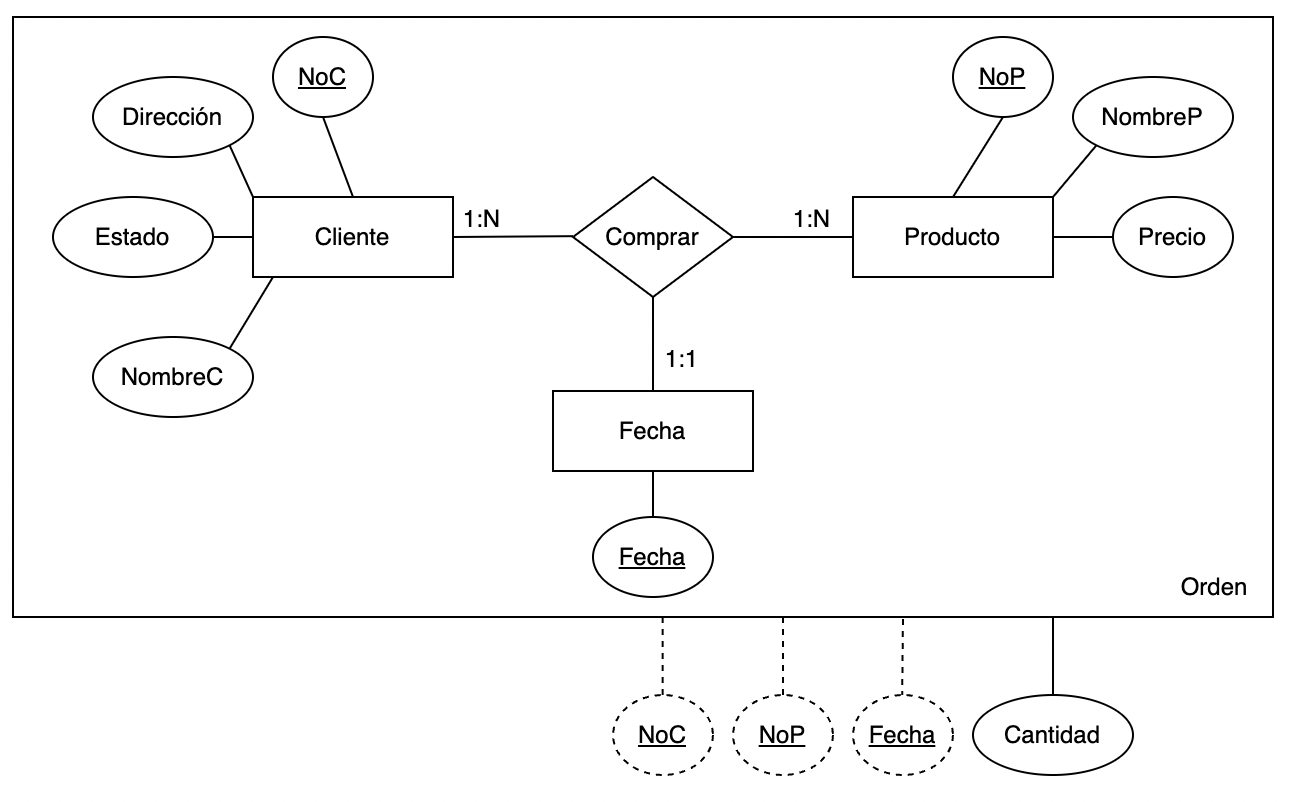
\includegraphics[scale=0.5]{bd.png}
	\end{figure}

	
\end{frame}

%------------------------------------------------

\begin{frame}[fragile]
	
	\frametitle{Iniciando con la sintaxis de la cláusula SELECT}
	
		\begin{lstlisting}[ language=SQL,
			deletekeywords={IDENTITY},
			deletekeywords={[2]INT},
			morekeywords={clustered},
			framesep=8pt,
			xleftmargin=40pt,
			framexleftmargin=40pt,
			frame=tb,
			framerule=0pt ]
SELECT * | <column_1>, <column_2>, ...
FROM <table_name>;
\end{lstlisting}

	\pause
	
	\ 
	
	\ 
	
	\begin{itemize}
		\item SELECT: Define columnas a tomar
		\item FROM: Define la tabla a consultar
	\end{itemize}

\end{frame}

%------------------------------------------------

\begin{frame}[fragile]
	
	\frametitle{La primera consulta}
	
	Sintaxis:
	\begin{lstlisting}[ language=SQL,
		deletekeywords={IDENTITY},
		deletekeywords={[2]INT},
		morekeywords={clustered},
		framesep=8pt,
		xleftmargin=40pt,
		framexleftmargin=40pt,
		frame=tb,
		framerule=0pt ]
SELECT * | <column_1>, <column_2>, ...
FROM <table_name>;
\end{lstlisting}

	\ 
	
		
	Construya una consulta para ver la información del \textbf{cliente}.
	
	\pause

	\begin{columns}[t]
		\column{0.4\textwidth}
		\begin{lstlisting}[ language=SQL,
			deletekeywords={IDENTITY},
			deletekeywords={[2]INT},
			morekeywords={clustered},
			framesep=8pt,
			xleftmargin=40pt,
			framexleftmargin=40pt,
			frame=tb,
			framerule=0pt ]
SELECT *
FROM cliente;
\end{lstlisting}
	
	\column{0.6\textwidth}
	
		\begin{lstlisting}[ language=SQL,
		deletekeywords={IDENTITY},
		deletekeywords={[2]INT},
		morekeywords={clustered},
		framesep=8pt,
		xleftmargin=40pt,
		framexleftmargin=40pt,
		frame=tb,
		framerule=0pt ]
SELECT NoC, NombreC, Dirección, Estado
FROM cliente;
\end{lstlisting}
	
	\end{columns}
	
	\pause
	
	\ 
	
	Dos consultas que generan el mismo resutado, pero una aprovecha el ``azúcar'' sintáctico de SQL.
	
	\pause
	
	\ 
	
	\textcolor{codepurple}{¿Cómo elegir las filas a mostrar?}
			
\end{frame}

%------------------------------------------------

\begin{frame}[fragile]
	
	\frametitle{Seleccionando filas}
	
	Sintaxis:
	\begin{lstlisting}[ language=SQL,
		deletekeywords={IDENTITY},
		deletekeywords={[2]INT},
		morekeywords={clustered},
		framesep=8pt,
		xleftmargin=40pt,
		framexleftmargin=40pt,
		frame=tb,
		framerule=0pt ]
SELECT * | <column_1>, <column_2>, ...
FROM <table_name>
WHERE <constraint_expresion>;
\end{lstlisting}

	\ 
	
	\pause 
	
	Posibles operadores a usar: 
	\begin{itemize}
	
		\item Lógicos: $AND$, $OR$, $NOT$
		
		\item Relacionales: $<$, $<=$, $>=$, $>$, $=$, $<>$
		
		
		\pause
		
		\ 
		
		Construya una consulta para obtener todos los productos cuyo precio sea menor o igual a $10$, o mayor que $2000$.
		
		\pause
		
		\ 
			\begin{lstlisting}[ language=SQL,
			deletekeywords={IDENTITY},
			deletekeywords={[2]INT},
			morekeywords={clustered},
			framesep=8pt,
			xleftmargin=40pt,
			framexleftmargin=40pt,
			frame=tb,
			framerule=0pt ]
SELECT NombreP, Precio
FROM producto
WHERE Precio <= 10 OR Precio > 2000; 
\end{lstlisting}
		
	\end{itemize}
	
\end{frame}

%------------------------------------------------

\begin{frame}[fragile]
	
	\frametitle{Seleccionando filas}
	
	Sintaxis:
	\begin{lstlisting}[ language=SQL,
		deletekeywords={IDENTITY},
		deletekeywords={[2]INT},
		morekeywords={clustered},
		framesep=8pt,
		xleftmargin=40pt,
		framexleftmargin=40pt,
		frame=tb,
		framerule=0pt ]
SELECT expresion
FROM table_name
WHERE constraint_expresion;
\end{lstlisting} 
	
	Posibles operadores a usar: 
	\begin{itemize}
		
		\item Especiales: $IN$, $LIKE$, $BETWEEN$, $IS\ NULL$
		
		\pause 
		
		\ 
		
		Construya una consulta para obtener todos los clientes que pertenezcan a ``Ohio'', ``Nevada'' o ``Misisipi''.
		
		\pause
		
		\begin{columns}[t]
			\column{0.5\textwidth}
			\begin{lstlisting}[ language=SQL,
				deletekeywords={IDENTITY},
				deletekeywords={[2]INT},
				morekeywords={clustered},
				framesep=8pt,
				xleftmargin=40pt,
				framexleftmargin=40pt,
				frame=tb,
				framerule=0pt ]
SELECT NombreC 
FROM cliente 
WHERE Estado IN ('Ohio', 'Nevada', 'Misisipi');
\end{lstlisting}
			
			\column{0.5\textwidth}
			\begin{lstlisting}[ language=SQL,
				deletekeywords={IDENTITY},
				deletekeywords={[2]INT},
				morekeywords={clustered},
				framesep=8pt,
				xleftmargin=40pt,
				framexleftmargin=40pt,
				frame=tb,
				framerule=0pt ]
SELECT NombreC 
FROM cliente 
WHERE Estado = 'Ohio' OR  Estado = 'Nevada' OR Estado =  'Misisipi';
\end{lstlisting}
			
		\end{columns}
		
	\end{itemize}
	
\end{frame}

%------------------------------------------------

\begin{frame}[fragile]
	
	\frametitle{Seleccionando filas}
	
	Sintaxis:
	\begin{lstlisting}[ language=SQL,
		deletekeywords={IDENTITY},
		deletekeywords={[2]INT},
		morekeywords={clustered},
		framesep=8pt,
		xleftmargin=40pt,
		framexleftmargin=40pt,
		frame=tb,
		framerule=0pt ]
SELECT <expresion>
FROM <table_name>
WHERE <constraint_expresion>;
\end{lstlisting} 
	
	Posibles operadores a usar: 
	\begin{itemize}
		
		\item Especiales: $IN$, $LIKE$, $BETWEEN$, $IS\ NULL$
		
		\pause 
		
		\ 
		
		Construya una consulta para obtener todos los clientes cuyo nombre comience con la letra ``\texttt{I}'' y culmine con al menos cuatro letras, donde las dos últimas tienen que ser ``\texttt{er}''. La columna de la tabla resultante tiene que llamarse ``Cliente Especial I-er''.
		
		\pause
		
			\begin{lstlisting}[ language=SQL,
				deletekeywords={IDENTITY},
				deletekeywords={[2]INT},
				morekeywords={clustered},
				framesep=8pt,
				xleftmargin=40pt,
				framexleftmargin=40pt,
				frame=tb,
				framerule=0pt ]
SELECT NombreC AS `Cliente Especial I-er`
FROM cliente 
WHERE NombreC LIKE 'I%_er';
\end{lstlisting}
			
	\end{itemize}
	
\end{frame}

%------------------------------------------------

\begin{frame}[fragile]
	
	\frametitle{Desglosando el comando LIKE}
	
			\begin{lstlisting}[ language=SQL,
			deletekeywords={IDENTITY},
			deletekeywords={[2]INT},
			morekeywords={clustered},
			framesep=8pt,
			xleftmargin=40pt,
			framexleftmargin=40pt,
			frame=tb,
			framerule=0pt ]
SELECT NombreC AS `Cliente Especial I-er`
FROM cliente 
WHERE NombreC LIKE 'I%_er';
\end{lstlisting}

	\ 
	
	El comando \textcolor{codepurple}{AS} brinda alias a columnas o tablas.
	
	\pause
	
	\ 
	
	Comodines de  \textcolor{codepurple}{LIKE}: 
	\begin{itemize}
		
		\item \textcolor{codepurple}{$\%$} Representa cero, uno o múltiples caracteres
		
		\item \textcolor{codepurple}{\textbf{$\_$}} \ \ Representa un solo caracter
					
	\end{itemize}
	
	\pause 
	
	\ 
	
	Existen otros comodines que permiten generalizar el comando y utilizarlo con expresiones regulares.
	
	\pause
	
	\ 
	
	\textcolor{red}{¿Cómo ordenar la relación resultante?}
	
\end{frame}

%------------------------------------------------

\begin{frame}[fragile]

	\frametitle{Ordenando los resultados}
	
	Construya una consulta para obtener todos los clientes, su dirección y su estado, pero ordenados de forma descendente por la dirección y el estado al que pertenecen.
	
	\pause
	
	\ 
	
	Sintaxis:
	\begin{lstlisting}[ language=SQL,
		deletekeywords={IDENTITY},
		deletekeywords={[2]INT},
		morekeywords={clustered},
		framesep=8pt,
		xleftmargin=40pt,
		framexleftmargin=40pt,
		frame=tb,
		framerule=0pt ]
SELECT <expresion>
FROM <table_name>
ORDER BY <field> [ASC|DESC], ...;
\end{lstlisting} 

	\pause
	
	\ 
	
	Solución:
	\begin{columns}[t]
		\column{0.5\textwidth}
		\begin{lstlisting}[ language=SQL,
			deletekeywords={IDENTITY},
			deletekeywords={[2]INT},
			morekeywords={clustered},
			framesep=8pt,
			xleftmargin=10pt,
			framexleftmargin=10pt,
			frame=tb,
			framerule=0pt ]
SELECT NombreC, Dirección, Estado 
FROM cliente 
ORDER BY Estado ASC, Dirección DESC;
\end{lstlisting} 
		
		\column{0.5\textwidth}
		\begin{lstlisting}[ language=SQL,
			deletekeywords={IDENTITY},
			deletekeywords={[2]INT},
			morekeywords={clustered},
			framesep=8pt,
			xleftmargin=10pt,
			framexleftmargin=10pt,
			frame=tb,
			framerule=0pt ]
SELECT NombreC, Dirección, Estado 
FROM cliente 
ORDER BY Estado, Dirección DESC;
\end{lstlisting} 
		
	\end{columns}
	
	\pause 
	
	\ 
	
	
	\textcolor{codepurple}{¿Cómo limitar el número de filas mostradas?}
	
\end{frame}

%------------------------------------------------

\begin{frame}[fragile]
	
	\frametitle{Limitando la cantidad de filas a mostrar}
	
	Sintaxis:
	\begin{lstlisting}[ language=SQL,
		deletekeywords={IDENTITY},
		deletekeywords={[2]INT},
		morekeywords={clustered},
		framesep=8pt,
		xleftmargin=40pt,
		framexleftmargin=40pt,
		frame=tb,
		framerule=0pt ]
SELECT * | <column_1>, <column_2>, ...
FROM <table_name>
LIMIT <number>;
\end{lstlisting}
	
	\pause 
	
	\ 
	
	\ 
	
	Con la siguiente consulta, se muestran solo 10 filas 
	
	\begin{lstlisting}[ language=SQL,
		deletekeywords={IDENTITY},
		deletekeywords={[2]INT},
		morekeywords={clustered},
		framesep=8pt,
		xleftmargin=40pt,
		framexleftmargin=40pt,
		frame=tb,
		framerule=0pt ]
SELECT *
FROM cliente
LIMIT 10;
\end{lstlisting}
	
	\pause
	
	\ 
	
	\ 
	
	
	\textcolor{red}{¿Qué pasa si se quiere resumir la información?}
	

\end{frame}

%------------------------------------------------

\begin{frame}[fragile]

	\frametitle{Agrupando los resultados}
	
	Construya una consulta que muestre la cantidad de clientes por estado.
	
		\pause
	
	\ 
	
	Sintaxis:
	\begin{lstlisting}[ language=SQL,
		deletekeywords={IDENTITY},
		deletekeywords={[2]INT},
		morekeywords={clustered},
		framesep=8pt,
		xleftmargin=40pt,
		framexleftmargin=40pt,
		frame=tb,
		framerule=0pt ]
SELECT <expresion>
FROM <table_name>
GROUP BY <field_1> [, <field_2>, ...] ;
\end{lstlisting} 
	
	\pause
	
	\ 
	
	Solución:
		\begin{lstlisting}[ language=SQL,
		deletekeywords={IDENTITY},
		deletekeywords={[2]INT},
		morekeywords={clustered},
		framesep=8pt,
		xleftmargin=40pt,
		framexleftmargin=40pt,
		frame=tb,
		framerule=0pt ]
SELECT Estado, COUNT(NoC) AS Cantidad
FROM cliente 
GROUP BY Estado;
\end{lstlisting} 
	
\end{frame}

%------------------------------------------------

\begin{frame}[fragile]
	
	\frametitle{Funciones útiles para resumir}
	
	\begin{itemize}
		
		\item COUNT() : Cuenta la cantidad de registros
		
		\item MAX() : Determina el valor máximo para un atributo
		
		\item MIN() : Determina el valor mínimo para un atributo
		
		\item SUM() : Suma los valores de un atributo
		
		\item AVG() : Calcula el promedio de los valores de un atributo
		
	\end{itemize}
	
	\ 
	
	\ 
	
	\pause
	
	Las funciones a utilizar por el uso de la cláusula \textcolor{codepurple}{GROUP BY} requieren un conjunto de valores dado por el nombre del atributo. En el caso de \textbf{COUNT}, no es necesario la definición de un atributo, basta con el uso de ``\textbf{*}''.
	
	\ 
	
	\ 
	
	\pause
	
	\textcolor{red}{¿Y si se quiere seleccionar algunas tuplas luego de agrupar?}
	
\end{frame}

%------------------------------------------------

\begin{frame}[fragile]

	\frametitle{Añadiendo condición al agrupar}

	Sintaxis:
	\begin{lstlisting}[ language=SQL,
		deletekeywords={IDENTITY},
		deletekeywords={[2]INT},
		morekeywords={clustered},
		framesep=8pt,
		xleftmargin=40pt,
		framexleftmargin=40pt,
		frame=tb,
		framerule=0pt ]
SELECT <expresion>
FROM <table_name>
GROUP BY <field_1> [, <field_2>, ...]
HAVING <constraint_expresion>;
\end{lstlisting}

	\pause 

	\ 

	Construya una consulta que muestre la cantidad de clientes por estado tal que su total sea menor que 5. 

	\  

	\pause 

	\begin{lstlisting}[ language=SQL,
		deletekeywords={IDENTITY},
		deletekeywords={[2]INT},
		morekeywords={clustered},
		framesep=8pt,
		xleftmargin=40pt,
		framexleftmargin=40pt,
		frame=tb,
		framerule=0pt ]
SELECT Estado, COUNT(NoC) AS Cantidad
FROM cliente 
GROUP BY Estado
HAVING COUNT(NoC) < 5;
\end{lstlisting}

	\pause
	
	\ 
	
	\textcolor{red}{Y si se quieren expresar alternativas, ¿qué cláusula me lo facilita?}

\end{frame}

%------------------------------------------------

\begin{frame}[fragile]
	
	\frametitle{Utilizando alternativas}
	
	La clásula  \textcolor{codepurple}{CASE} tiene un comportamiento similar al conocido \emph{if-then-else}. En caso de no tener definido ``else'' y no cumplirse ninguna condición, el retorno será \textbf{NULL}.
	
	\ 
	
	Sintaxis: 
	
	\begin{lstlisting}[ language=SQL,
		deletekeywords={IDENTITY},
		deletekeywords={[2]INT},
		morekeywords={clustered},
		framesep=8pt,
		xleftmargin=40pt,
		framexleftmargin=40pt,
		frame=tb,
		framerule=0pt ]
CASE
  WHEN condition_1 THEN result_1
  [WHEN condition_2 THEN result_2, 
  ...
  ELSE result]
END;
\end{lstlisting}
	
	
\end{frame}

%------------------------------------------------

\begin{frame}[fragile]
	
	\frametitle{Utilizando \emph{if-then-else}}
	
	Construya una consulta para conocer si el precio de un producto es barato, normal, caro o muy caro. 
	
	\begin{columns}[t]
		\column{0.5\textwidth}
		\begin{table}[]
			\begin{tabular}{|l|l|}
				\hline
				Etiqueta & Rango de precio \\ \hline \hline
				barato   & {[}0, 100)        \\ \hline
				normal   & {[}100, 1000)       \\ \hline
			\end{tabular}
		\end{table}
		
		\column{0.5\textwidth}
		
		\begin{table}[]
			\begin{tabular}{|l|l|}
				\hline
				Etiqueta   & Rango de precio \\ \hline \hline
				caro          & {[}1000, 2000)        \\ \hline
				muy caro & e.o.c       \\ \hline
			\end{tabular}
		\end{table}
		
	\end{columns}
	
	\pause
	
	\ 
	
	\begin{lstlisting}[ language=SQL,
		deletekeywords={IDENTITY},
		deletekeywords={[2]INT},
		morekeywords={clustered},
		framesep=8pt,
		xleftmargin=40pt,
		framexleftmargin=40pt,
		frame=tb,
		framerule=0pt ]
SELECT 
  NombreP as Producto, 
  CASE 
    WHEN Precio >= 0 AND Precio < 100 THEN 'barato'
    WHEN Precio >= 100 AND Precio < 1000 THEN 'normal'
    WHEN Precio >= 1000 AND Precio < 2000 THEN 'caro'
    ELSE 'muy caro'
  END AS `Tipo de precio`
FROM producto;
\end{lstlisting}
	
\end{frame}

%------------------------------------------------

{
	\setbeamertemplate{background canvas}
	{%
		
\includegraphics[width=\paperwidth,height=\paperheight]{sql_on_fire.jpg}
	}
	
	\begin{frame}
	\end{frame}
}

%------------------------------------------------

\begin{frame}{t}
	
	\frametitle{Recordando las tablas}
	
	\begin{figure}[h]
		\centering
		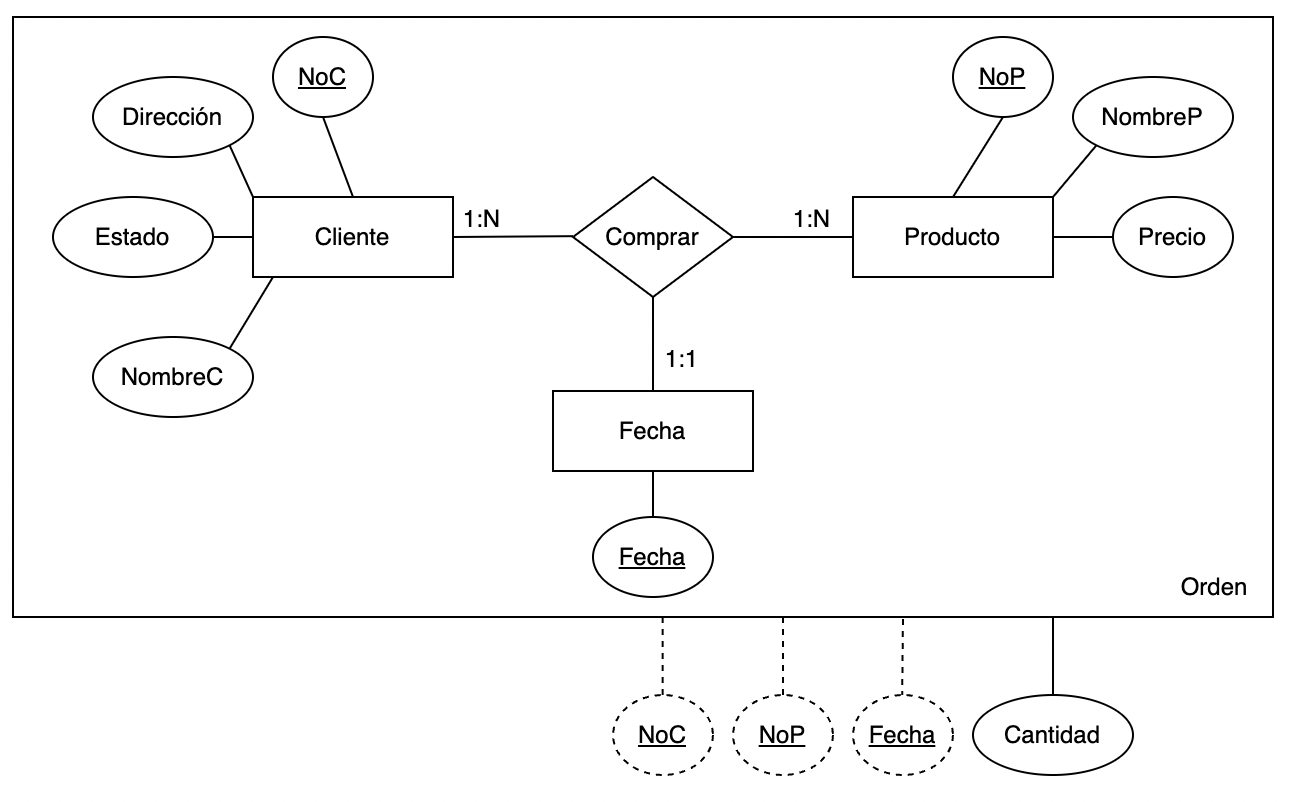
\includegraphics[scale=0.5]{bd.png}
	\end{figure}
	
	
\end{frame}

%------------------------------------------------

\begin{frame}[fragile]
	
		\frametitle{La cl\'ausula JOIN}
		
		La cláusula \textcolor{codepurple}{JOIN} permite relacionar varias tablas, usando las \emph{llaves foráneas} o bien columnas de referencias.
		
		\ 
		
		\ 
		
		\pause
		
		Sintaxis: 
		\begin{lstlisting}[ language=SQL,
			deletekeywords={IDENTITY},
			deletekeywords={[2]INT},
			morekeywords={clustered},
			framesep=8pt,
			xleftmargin=40pt,
			framexleftmargin=40pt,
			frame=tb,
			framerule=0pt ]
SELECT <expresion>
FROM <table_name_1>
  JOIN <table_name_2>
  ON <table_name_1>.<field_1> = <table_name_2>.<field_2>;
\end{lstlisting}
		
\end{frame}

%------------------------------------------------

\begin{frame}[fragile]
	
	\frametitle{Tipos de JOIN}
	
	\begin{center}
		
		\textcolor{codepurple}{INNER JOIN}
		
		\ 
		
		Obtiene todos los registros, siempre y cuando exista una coincidencia de los valores de las columnas definidas de ambas tablas.
		
		\begin{venndiagram2sets}[
			labelA={ }, labelOnlyA={Tabla1}, 
			labelB={ }, labelOnlyB={Tabla2}, 
			showframe=false]
			\fillACapB
		\end{venndiagram2sets}
		
	\end{center}
	
\end{frame}

%------------------------------------------------

\begin{frame}[fragile]
	
	\frametitle{Tipos de JOIN}
	
	\begin{center}
		\textcolor{codepurple}{INNER JOIN}
	\end{center}
	
	\ 
		
	Construya una consulta que muestre el cliente y la fecha en que efectuó alguna compra.
		
		\pause 
		
		\ 
		
		\ 
		
		\begin{lstlisting}[ language=SQL,
			deletekeywords={IDENTITY},
			deletekeywords={[2]INT},
			morekeywords={clustered},
			framesep=8pt,
			xleftmargin=40pt,
			framexleftmargin=40pt,
			frame=tb,
			framerule=0pt ]
SELECT 
  NombreC as Cliente, 
  Fecha
FROM orden 
  JOIN cliente
    ON orden.NoC = cliente.NoC;
\end{lstlisting}
				
\end{frame}

%------------------------------------------------

\begin{frame}[fragile]
	
	\frametitle{Tipos de JOIN}
	
	\begin{center}
	
		\textcolor{codepurple}{LEFT (OUTER) JOIN}
		
		\ 
		
		Obtiene todos los registros de la tabla que aparece en el \textcolor{codepurple}{FROM}, conocida como tabla izquierda (\textbf{Tabla1}). Los registros de la tabla posterior al \textcolor{codepurple}{JOIN}, conocida como tabla derecha (\textbf{Tabla2}), se añaden si existe alguna coincidencia de los valores de las columnas definidas. En caso contrario, se mostrará \textcolor{codepurple}{NULL}.
		
		\begin{venndiagram2sets}[
			labelA={ }, labelOnlyA={Tabla1}, 
			labelB={ }, labelOnlyB={Tabla2}, 
			showframe=false]
			\fillA
		\end{venndiagram2sets}
		
	\end{center}

\end{frame}
	
%------------------------------------------------

\begin{frame}[fragile]
	
	\frametitle{Tipos de JOIN}
	
	\begin{center}
		\textcolor{codepurple}{LEFT (OUTER) JOIN}
	\end{center}
	
	\ 
	
	Construya una consulta que muestre el cliente y la fecha en que efectuó alguna compra. Deben de aparecer también aquellos clientes que no hayan efectuado compra alguna.
	
	\pause 
	
	\ 
	
	\ 
	
	\begin{lstlisting}[ language=SQL,
		deletekeywords={IDENTITY},
		deletekeywords={[2]INT},
		morekeywords={clustered},
		framesep=8pt,
		xleftmargin=40pt,
		framexleftmargin=40pt,
		frame=tb,
		framerule=0pt ]
SELECT 
  NombreC AS Cliente, 
  Fecha
FROM cliente
  LEFT JOIN orden 
    ON orden.NoC = cliente.NoC;
\end{lstlisting}
	
\end{frame}

%------------------------------------------------

\begin{frame}[fragile]
	
	\frametitle{Tipos de JOIN}
	
	\begin{center}
	
		\textcolor{codepurple}{RIGHT (OUTER) JOIN}
		
		\ 
		
			Obtiene todos los registros de la tabla posterior al \textcolor{codepurple}{JOIN}, conocida como tabla derecha (\textbf{Tabla2}). Los registros de la tabla que aparece en el \textcolor{codepurple}{FROM}, conocida como tabla izquierda (\textbf{Tabla1}), se añaden si existe alguna coincidencia de los valores de las columnas definidas. En caso contrario, se mostrará \textcolor{codepurple}{NULL}.
		
		\begin{venndiagram2sets}[
			labelA={ }, labelOnlyA={Tabla1}, 
			labelB={ }, labelOnlyB={Tabla2}, 
			showframe=false]
			\fillB
		\end{venndiagram2sets}
		
	\end{center}
	
	\pause
	
	\ 
	
	\textcolor{red}{¿Qué devuelve la consulta anterior si se emplea \textcolor{codepurple}{RIGHT JOIN}?}
	
		
\end{frame}

%------------------------------------------------

\begin{frame}[fragile]
	
	\frametitle{Tipos de JOIN}
	
	\begin{center}
	
		\textcolor{codepurple}{FULL (OUTER) JOIN}
		
		\ 
		
		Combina los resultados de los \emph{joins LEFT} y \emph{RIGHT}. Alternativamente, aparecerá \textcolor{codepurple}{NULL} cada registro de la tabla, cuando no haya coincidencia.		
		
		\begin{venndiagram2sets}[
			labelA={ }, labelOnlyA={Tabla1}, 
			labelB={ }, labelOnlyB={Tabla2}, 
			showframe=false]
			\fillA
			\fillB
		\end{venndiagram2sets}
	
	\end{center}
	
	\pause
	
	\ 
	
	\textcolor{red}{¿Qué devuelve la consulta anterior si se emplea \textcolor{codepurple}{FULL JOIN}?}
		
\end{frame}

%------------------------------------------------

\begin{frame}[fragile]
	
	\frametitle{¿Qué son las subconsultas?}
	
	\begin{itemize}
		
		\item En ocasiones, se necesita definir consultas anidadas, o sea, consultas dentro de otra consulta. Esto se conoce como \textbf{subconsultas}. 
		
		\item Las subconsultas pueden definirse en las cláusulas: \textcolor{codepurple}{SELECT}, \textcolor{codepurple}{FROM}, \textcolor{codepurple}{WHERE}, \textcolor{codepurple}{HAVING}.
		
		\item Existen reglas al utilizar subconsultas.
		
	\end{itemize}
		
\end{frame}

%------------------------------------------------

\begin{frame}[fragile]
	
	\frametitle{Trabajando con subconsultas}
	
	Construya una consulta para obtener los productos más baratos, teniendo en cuenta que: 
 
    \vspace{-4mm}
	
	\begin{columns}[t]
		\column{0.5\textwidth}
		\begin{table}[]
			\begin{tabular}{|l|l|}
				\hline
				Etiqueta & Rango de precio \\ \hline \hline
				barato   & {[}0, 100)        \\ \hline
				normal   & {[}100, 1000)       \\ \hline
			\end{tabular}
		\end{table}
		
		\column{0.5\textwidth}
		
		\begin{table}[]
			\begin{tabular}{|l|l|}
				\hline
				Etiqueta   & Rango de precio \\ \hline \hline
				caro          & {[}1000, 2000)        \\ \hline
				muy caro & e.o.c       \\ \hline
			\end{tabular}
		\end{table}
		
	\end{columns}
	
	\pause
	
	\begin{lstlisting}[ language=SQL,
		deletekeywords={IDENTITY},
		deletekeywords={[2]INT},
		morekeywords={clustered},
		framesep=8pt,
		xleftmargin=40pt,
		framexleftmargin=40pt,
		frame=tb,
		framerule=0pt ]
SELECT Producto
FROM ( 
    SELECT NombreP AS Producto, 
        CASE WHEN Precio >= 0 AND Precio < 100 THEN 'barato'
             WHEN Precio >= 100 AND Precio < 1000 THEN 'normal'
             WHEN Precio >= 1000 AND Precio < 2000 THEN 'caro'
             ELSE 'muy caro'
        END AS `Tipo de precio`
    FROM producto
  ) 
WHERE `Tipo de precio` = 'barato';  
\end{lstlisting}
		
\end{frame}

%------------------------------------------------

\begin{frame}
	
	\begin{figure}[h]
		\centering
		
\includegraphics[scale=0.5]{mucho.png}
	\end{figure}
	
\end{frame}

%------------------------------------------------

\begin{frame}

	\frametitle{Orden de ejecución de las cláusulas}
	
	\begin{figure}[h]
		\centering
		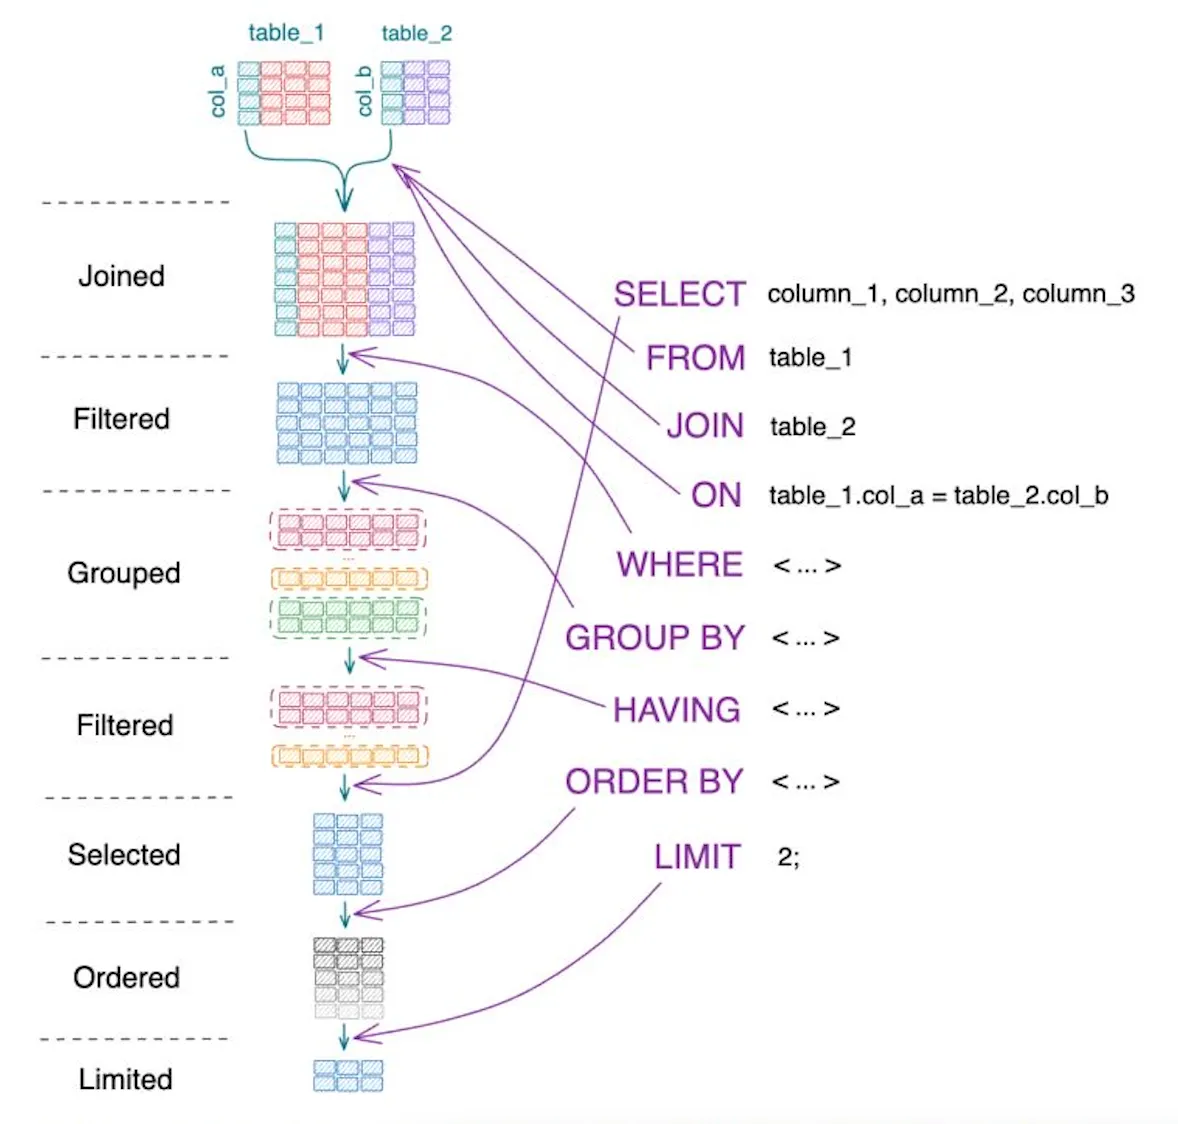
\includegraphics[scale=0.2]{orden.jpg}
	\end{figure}

\end{frame}

%------------------------------------------------

\begin{frame}
	
	\frametitle{Resumen de cláusulas}

\begin{table}
	\begin{tabular}{|l|c|m{6cm}|c|}
		\hline 
		Cláusula & \multicolumn{1}{l|}{?`Es obligatoria?} & ?`Qu\'e hace? & \multicolumn{1}{l|}{?`Qu\'e modifica?} \\ \hline \hline
		SELECT & Sí & Identifica las columnas a mostrar en la relación & - \\ \hline
		FROM & Sí & Determina la fuente de datos & - \\ \hline
		WHERE & No & Restringe los registros de la fuente de datos a utilizar & FROM (y JOIN) \\ \hline
		JOIN & No & Determina otras fuentes de datos y cómo relacionarlas con la establecida en el FROM & - \\ \hline
		GROUP BY & No & Agrupa los registros ``similares''& - \\ \hline
		HAVING & No & Restringe los grupos & GROUP BY \\ \hline
		ORDER BY & No & Ordena los registros & - \\ \hline
		LIMIT & No & Limita la cantidad de registros a mostrar & - \\ \hline
	\end{tabular}
\end{table}




\end{frame}

%------------------------------------------------